\chapter{KỸ THUẬT VÀ KẾT QUẢ PHÂN CỤM}

\section{Giảm chiều dữ liệu bằng PCA}

\subsection{Thiết lập PCA}

Dữ liệu sau chuẩn hóa được giảm từ 17 chiều xuống 2 thành phần chính để trực quan hóa và huấn luyện phân cụm:
\begin{equation}
X_{n \times 17} \rightarrow X_{n \times 2}
\end{equation}

\begin{table}[H]
\centering
\caption{Tỷ lệ phương sai được giữ lại bởi PCA}
\begin{tabular}{|l|r|r|}
\hline
\textbf{Thành phần} & \textbf{Variance Ratio} & \textbf{Cộng dồn} \\
\hline
PC1 & 34.5\% & 34.5\% \\
\hline
PC2 & 22.0\% & 56.46\% \\
\hline
\end{tabular}
\end{table}

\textbf{Nhận xét:}
\begin{itemize}
    \item Hai thành phần đầu giữ lại 56.46\% phương sai, đủ để phản ánh cấu trúc hành vi chính
    \item PC1 chủ yếu liên quan đến cường độ sử dụng tín dụng (BALANCE, PURCHASES)
    \item PC2 phản ánh xu hướng rút tiền mặt và tần suất giao dịch
\end{itemize}

\section{Xác định số cụm tối ưu}

\begin{figure}[H]
\centering
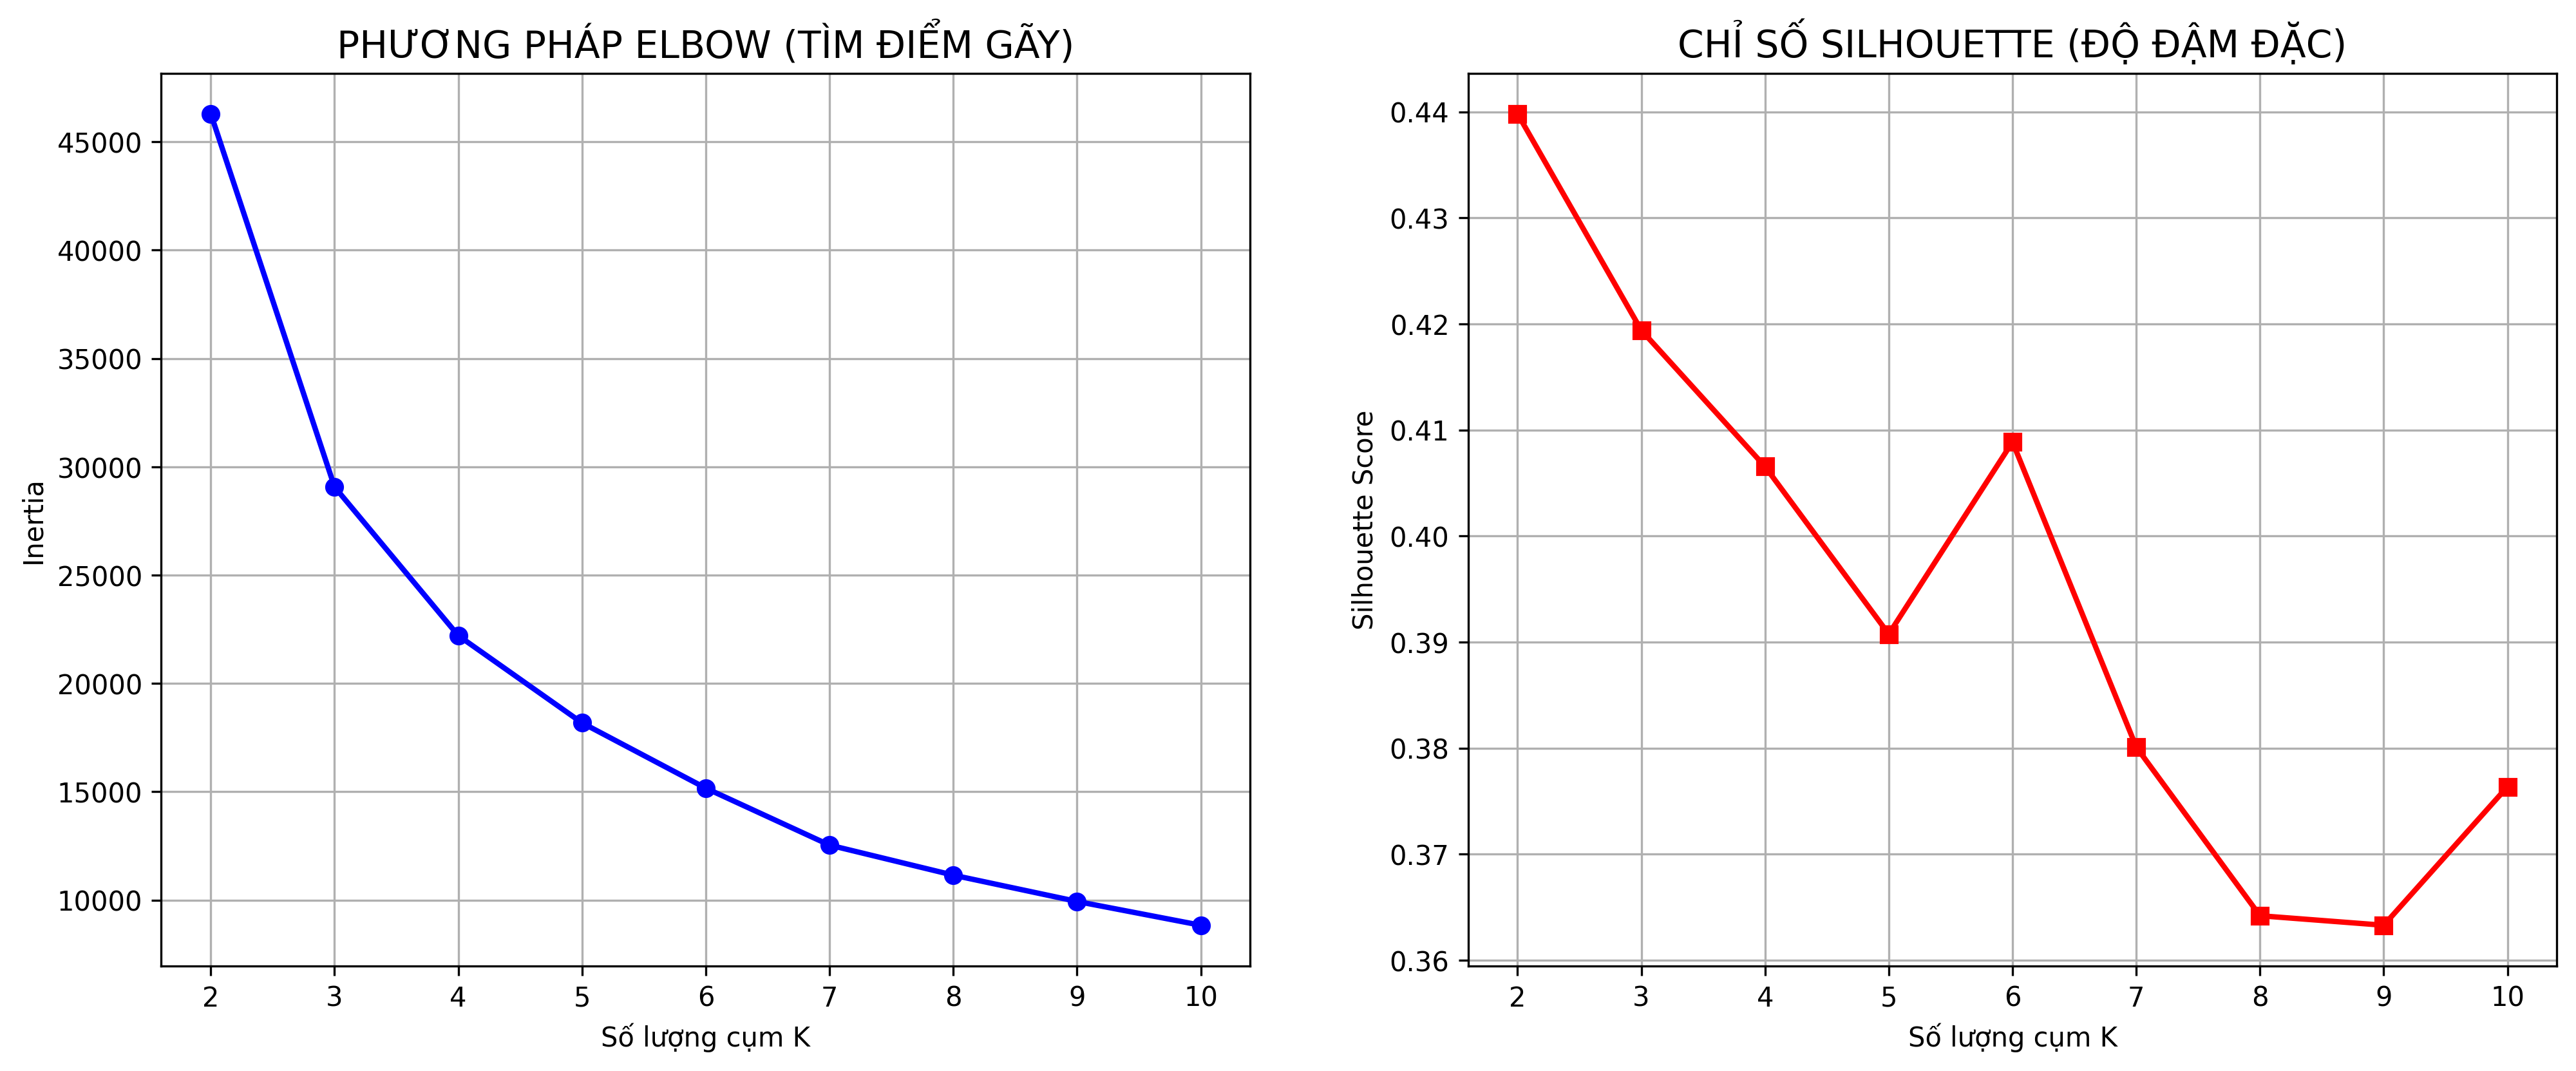
\includegraphics[width=0.9\textwidth]{evaluation_metrics.png}
\caption{Elbow và Silhouette theo số cụm}
\label{fig:evaluation_metrics}
\end{figure}

\textbf{Kết luận lựa chọn K:}
\begin{itemize}
    \item Elbow Method cho điểm gãy rõ tại $K=4$
    \item Silhouette tại $K=4$ đạt 0.215 (mức tách cụm vừa phải)
    \item K=4 được chọn vì cân bằng giữa chất lượng thống kê và khả năng hành động trong kinh doanh
\end{itemize}

\section{K-means với K=4}

\subsection{Thiết lập mô hình}

\begin{itemize}
    \item Thuật toán: K-means++
    \item Số cụm: 4
    \item n\_init: 10
    \item max\_iter: 300
    \item Số vòng lặp hội tụ: 19
\end{itemize}

\subsection{Đánh giá mô hình}

\begin{table}[H]
\centering
\caption{Các độ đo đánh giá tại K=4}
\begin{tabular}{|l|r|}
\hline
\textbf{Độ đo} & \textbf{Giá trị} \\
\hline
Silhouette Score & 0.215 \\
\hline
Davies-Bouldin Index & 1.64 \\
\hline
Calinski-Harabasz Index & 2,335 \\
\hline
Inertia & 85,335 \\
\hline
\end{tabular}
\end{table}

\subsection{Kiểm định độ ổn định của kết quả K-means}

Để tăng độ tin cậy học thuật, mô hình được chạy lặp lại 30 lần với các giá trị \texttt{random\_state} khác nhau (0--29), giữ nguyên toàn bộ pipeline tiền xử lý (median imputation, \texttt{log1p}, \texttt{StandardScaler}) và siêu tham số K-means (K=4, \texttt{n\_init}=10, \texttt{max\_iter}=300).

\begin{table}[H]
\centering
\caption{Độ ổn định của các chỉ số qua 30 lần chạy}
\begin{tabular}{|l|r|r|r|}
\hline
\textbf{Chỉ số} & \textbf{Trung bình} & \textbf{Độ lệch chuẩn} & \textbf{Khoảng giá trị} \\
\hline
Silhouette & 0.2154 & 0.0006 & [0.2150; 0.2187] \\
\hline
Davies-Bouldin & 1.6419 & 0.0029 & [1.6364; 1.6551] \\
\hline
Calinski-Harabasz & 2334.52 & 1.50 & [2326.59; 2334.82] \\
\hline
Inertia & 85339.96 & 24.09 & [85209.59; 85346.56] \\
\hline
Số vòng lặp hội tụ & 19.50 & -- & [11; 34] \\
\hline
ARI cặp đôi giữa các lần chạy & 0.9695 & 0.0827 & [0.6581; 1.0000] \\
\hline
\end{tabular}
\end{table}

\textbf{Diễn giải:}
\begin{itemize}
    \item Biến thiên của Silhouette, DBI, CHI và Inertia rất nhỏ, cho thấy chất lượng phân cụm ổn định theo khởi tạo ngẫu nhiên.
    \item ARI trung bình cao (0.9695) cho thấy cấu trúc phân cụm nhất quán ở đa số lần chạy.
    \item Một số cặp lần chạy có ARI thấp hơn (min = 0.6581), phản ánh có mức dao động cục bộ do dữ liệu có vùng chồng chéo giữa các cụm.
\end{itemize}

\subsection{Quy mô các cụm}

\begin{table}[H]
\centering
\caption{Phân bố khách hàng theo cụm K-means}
\begin{tabular}{|c|r|r|p{6cm}|}
\hline
\textbf{Cụm} & \textbf{Số lượng} & \textbf{Tỷ lệ} & \textbf{Đặc trưng nổi bật} \\
\hline
0 & 1,504 & 16.8\% & BALANCE cao, CASH\_ADVANCE rất cao, thanh toán đầy đủ thấp \\
\hline
1 & 2,206 & 24.6\% & PURCHASES cao nhất, thanh toán tốt, CASH\_ADVANCE rất thấp \\
\hline
2 & 2,758 & 30.8\% & Mức sử dụng thấp trên hầu hết biến, tiềm năng kích hoạt \\
\hline
3 & 2,482 & 27.7\% & Phụ thuộc rút tiền mặt, PURCHASES rất thấp, rủi ro tín dụng cao \\
\hline
\textbf{Tổng} & \textbf{8,950} & \textbf{100\%} & - \\
\hline
\end{tabular}
\end{table}

\section{Phân tích chi tiết 4 cụm}

\subsection{Cụm 0: Khách hàng rủi ro cao}

\begin{itemize}
    \item BALANCE: \$3,187 (cao hơn trung bình 103.7\%)
    \item CASH\_ADVANCE: \$2,551 (cao hơn trung bình 160.6\%)
    \item PRC\_FULL\_PAYMENT: 3.66\% (rất thấp)
\end{itemize}

\textbf{Diễn giải:} Nhóm này có xu hướng sử dụng hạn mức để rút tiền mặt và trả nợ không đầy đủ, cần ưu tiên quản trị rủi ro.

\subsection{Cụm 1: Khách hàng VIP (Premium/VIP Customers)}

\begin{itemize}
    \item PURCHASES: \$2,579 (cao nhất)
    \item PAYMENTS: \$2,492 (cao)
    \item CASH\_ADVANCE: \$40 (rất thấp)
    \item PRC\_FULL\_PAYMENT: 23.80\% (cao)
\end{itemize}

\textbf{Diễn giải:} Đây là nhóm giá trị cao, hành vi sử dụng thẻ lành mạnh, phù hợp chiến lược giữ chân và bán chéo.

\subsection{Cụm 2: Khách hàng ít sử dụng}

\begin{itemize}
    \item BALANCE: \$249
    \item PURCHASES: \$443
    \item CASH\_ADVANCE: \$24
    \item PRC\_FULL\_PAYMENT: 25.74\%
\end{itemize}

\textbf{Diễn giải:} Nhóm quy mô lớn nhất nhưng mức sử dụng thấp; có thể tăng doanh thu nếu kích hoạt đúng cách.

\subsection{Cụm 3: Khách hàng rút tiền mặt}

\begin{itemize}
    \item CASH\_ADVANCE: \$1,921
    \item PURCHASES: \$30
    \item PRC\_FULL\_PAYMENT: 3.46\%
\end{itemize}

\textbf{Diễn giải:} Nhóm có rủi ro tín dụng cao do phụ thuộc rút tiền mặt và khả năng trả nợ thấp.

\section{Đối chiếu DBSCAN}

Sử dụng DBSCAN với eps=0.5 và min\_samples=10:
\begin{itemize}
    \item Số cụm tìm thấy: 9
    \item Số điểm dị biệt: 8,486 (94.82\%)
\end{itemize}

\textbf{Kết luận đối chiếu:} Với bộ tham số này, DBSCAN không phù hợp cho bài toán phân khúc khách hàng trong dữ liệu hiện tại. K-means vẫn là lựa chọn chính cho báo cáo.

\section{Kết luận chương}

\begin{itemize}
    \item K-means với K=4 tạo ra 4 nhóm khách hàng có ý nghĩa kinh doanh rõ ràng
    \item Các cụm thể hiện tốt hai trục hành vi chính: chi tiêu và phụ thuộc rút tiền mặt
    \item Kết quả là cơ sở trực tiếp cho chương khuyến nghị kinh doanh
\end{itemize}
